\documentclass[12pt, a4paper]{article}

\usepackage{comment}
\usepackage{ragged2e}
\usepackage{amsmath}
\usepackage{dcolumn}
\usepackage{booktabs}
\usepackage{pdflscape}
\usepackage{graphicx}
\usepackage{placeins}
\usepackage{dcolumn}
\usepackage{xcolor}
\usepackage{booktabs}
\linespread{1.5}
\usepackage{subcaption}
\usepackage{amsmath}
\usepackage{hyperref}
\usepackage{multirow}
\usepackage{tikz}
\usepackage[title]{appendix}
\usetikzlibrary{decorations.pathreplacing}
\usepackage{booktabs}
\usepackage{tabularx}
\usepackage{datatool}
\hypersetup{
	colorlinks=false,
	linkcolor=black,
	filecolor=black,      
	urlcolor=black,
	citecolor = blue
}

\usepackage{natbib}
\usepackage{xepersian}
\settextfont{XB Niloofar}
\setdigitfont{XB Zar}
\newcommand{\paren}[1]{\scaleleftright[3cm]{\text{)}}{#1}{\text{(}}}
\def\sym#1{\ifmmode^{#1}\else\(^{#1}\)\fi}

\title{بتای حبابی }
%\subtitle{}
\author{
	مرتضی آقاجان‌زاده
	 \sym{*} 
	\qquad 
	مهدی حیدری 
	\sym{*} 
	 \\
	\sym{*} 
	\footnotesize  موسسه مطالعات پیشرفته تهران (تیاس) - دانشگاه خاتم
}

\date{
تیر 1400}




\begin{document}

\maketitle

\section{مقدمه}
\section{پیشینه پژوهش}
\section{روش‌شنای پژوهش}
\subsection{سبد‌های مرتب شده براساس بتا}
با توجه به ادبیات در ابتدای هر ماه با استفاده از داده‌های روزانه دوازده ماه گذشته بتای شرکت را محاسبه می‌کنیم. برای این کار بازده مازاد شرکت را بر بازده روازنه امروز و تا 5 روز قبل بازار برآورد می‌کنیم و ملاک بتای مورد مقایسه جمع 6 ضریب مطرح شده فوق می‌باشد. خلاصه آماری بتای محاسبه در جدول زیر نشان داده شده‌است:

\begin{table}[htbp]
	\caption{خلاصه آماری بتای ماهانه شرکت‌های مورد بررسی}
	\label{firstbetasummary}
	\begin{tabular}{c}
		مرتضی 
	\end{tabular}
\end{table}

در مرحله بعد نماد‌ها براساس بتا مرتب می‌شوند و به 10 سبد مجزا براساس بتا تقسیم می‌شوند که به ترتیب سبد شماره 1، شامل نماد‌های دارای کمترین بتا و سبد‌ شماره 10 دارای بیشترین مقادیر بتاست. درنتیجه در ابتدای هر ماه کلیه شرکت‌های بازار به 10 سبد تقسیم می‌شوند و بازده روزانه هر سبد براساس وزن اندازه بازار آن‌ها محاسبه می‌شود. سپس بتای سبد‌های ساخته شده با توجه به مدل قدم اول با استفاده از بازده روزانه آن‌ها محاسبه می‌شود. روند بازده سبد‌های ساخته شده در جدول و نمودار زیر نشان داده شده‌است:

		\begin{table}[htbp]
	\centering
	\caption{بازده متوسط سبد‌های مرتب شده براساس بتا}
\begin{LTR}	\resizebox{0.9\textwidth}{!}{
		\begin{tabular}{lrrrrrrrrrr}
	\toprule
	Portfolio & 1     & 2     & 3     & 4     & 5     & 6     & 7     & 8     & 9     & 10 \\
	\hline
	$ \beta $ & 0.64  & 0.68  & 0.71  & 0.82  & 0.96  & 1.21  & 1.13  & 1.26  & 1.38  & 1.77 \\
	12Return & 16.63 & 29.71 & 26.14 & 32.11 & 33.24 & 34.16 & 32.44 & 30.58 & 37.38 & 39.75 \\
	Mreturn & 1.73  & 2.47  & 2.32  & 2.76  & 3.38  & 2.69  & 2.91  & 2.53  & 3.43  & 3.67 \\
	Size  & 35    & 36    & 37    & 37    & 37    & 38    & 38    & 38    & 38    & 36 \\
	\bottomrule
	
	
\end{tabular}
		\label{tab:table1}	
	}
\end{LTR}
\end{table}
	\begin{figure}[htbp]
	\centering
	\caption{بازده متوسط سبد‌های مرتب شده براساس بتا}
	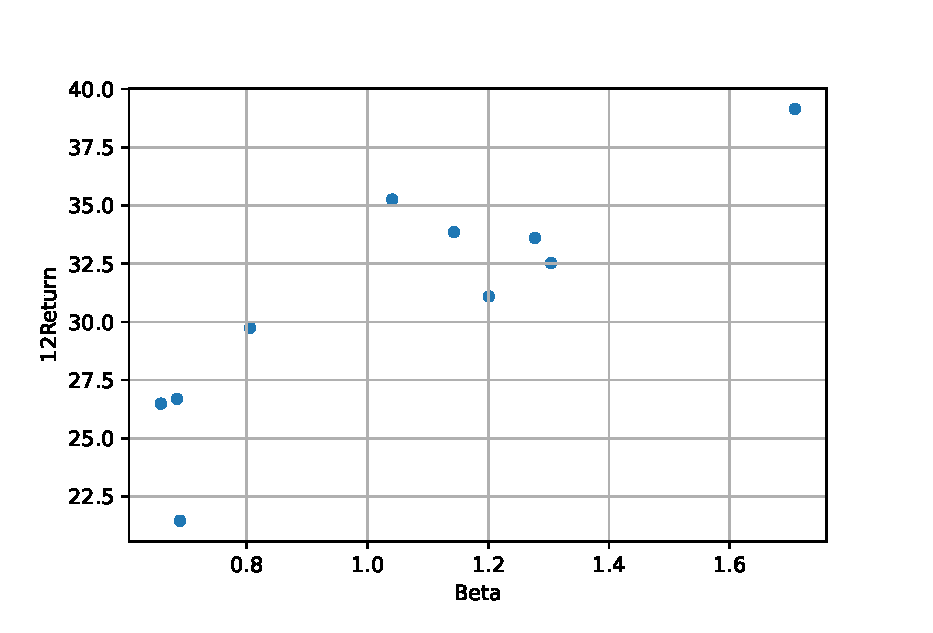
\includegraphics[width=0.7\linewidth]{BetaReturn10.eps}
	\label{fig:BetaReturn10}
\end{figure}
 همانطور که در نمودار و جدول فوق نشان داده شده‌است روند بیان شده در ادبیات مبنی بر بتای بالاتر به معنای ریسک بیشتر و به تبع آن بازده بیشتر است تایید شده‌است که بر خلاف نتایج بیان شده در مقاله 
 \cite{hong2016speculative}
 است. 
 در ادامه با توجه به مدل تئوری بیان شده در مقاله فوق نماد‌ها را به دو دسته حبابی و غیرحبابی تقسیم می‌کند. با توجه به شیوه مقاله سهام به دسته حبابی تعلق پیدا می‌کند چنانچه مقدار 
 $ \frac{\hat{\beta}_i}{\hat{\sigma}^2_i} $
 از میانه همین نسبت در میان نماد‌ها بیشتر باشد. شیوه برآورد و محاسبه بازده و بتای مانند قسمت قبل است. نتایج براساس دسته بندی نماد ها به دو دسته عبارتند از:
 \begin{table}[htbp]
 	\centering
 	\caption{بازده متوسط دو دسته سبد تعریف شده }
 	\begin{LTR}
 	\resizebox{0.7\textwidth}{!}{
 		\begin{tabular}{lcccccccccc}
	\toprule
	& 1     & 2     & 3     & 4     & 5     & 6     & 7     & 8     & 9     & 10 \\
	\midrule
	& \multicolumn{10}{c}{Nonspeculative} \\
	\midrule
	
	$\beta$  & 0.69  & 0.74  & 0.71  & 0.62  & 0.84  & 0.73  & 0.91  & 1.19  & 1.16  & 1.30 \\
	\multicolumn{1}{l}{12Return} & 50.07 & 42.39 & 53.00 & 59.10 & 64.57 & 43.80 & 55.05 & 71.15 & 57.46 & 56.05 \\
	\multicolumn{1}{l}{Mreturn} & 3.42  & 2.45  & 3.79  & 3.64  & 4.65  & 2.67  & 3.73  & 4.81  & 3.71  & 3.26 \\
	\multicolumn{1}{l}{Size} & 17    & 18    & 18    & 18    & 18    & 19    & 19    & 19    & 18    & 18 \\
	\midrule
	& \multicolumn{10}{c}{Speculative} \\
	\midrule
	$\beta$  & 0.69  & 0.91  & 0.90  & 1.10  & 1.14  & 1.05  & 1.26  & 1.24  & 1.40  & 1.58 \\
	\multicolumn{1}{l}{12Return} & 43.47 & 70.68 & 58.81 & 42.64 & 50.55 & 65.41 & 64.54 & 48.93 & 53.07 & 70.40 \\
	\multicolumn{1}{l}{Mreturn} & 3.07  & 4.91  & 4.23  & 2.42  & 3.23  & 4.38  & 3.95  & 3.24  & 3.43  & 4.75 \\
	\multicolumn{1}{l}{Size} & 18    & 18    & 19    & 19    & 19    & 19    & 19    & 19    & 19    & 19 \\
	
	\bottomrule
	
	
\end{tabular}%
 		\label{tab:table2}	
 	}
 	\end{LTR}
 \end{table}


\begin{figure}[htbp]
\centering
\caption{بازده متوسط سبد‌های مرتب شده براساس بتا}
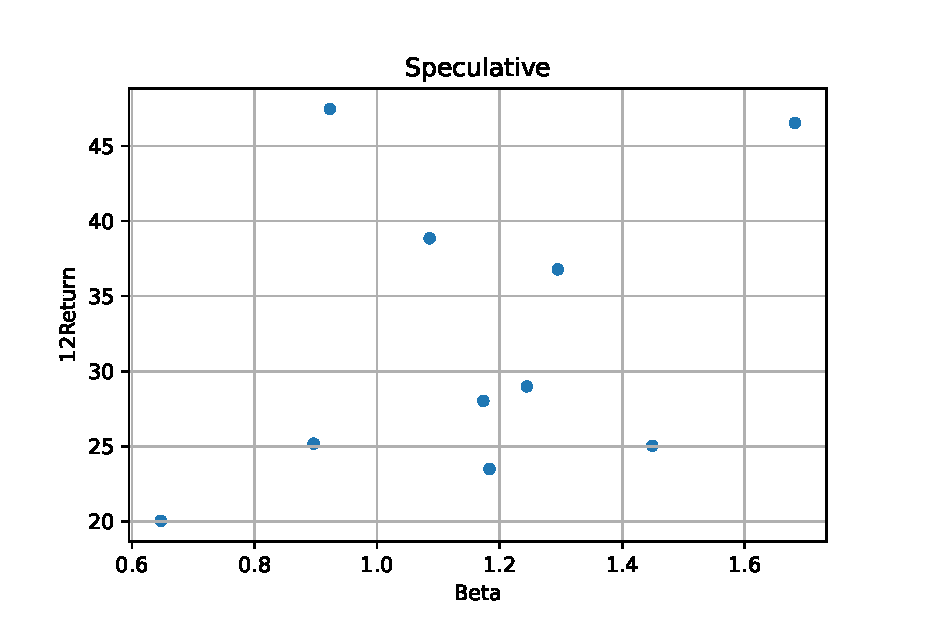
\includegraphics[width=0.7\linewidth]{SpeculativeBetaReturn10.eps}
\label{fig:SpeculativeBetaReturn10}
\end{figure}

\begin{figure}[htbp]
\centering
\caption{بازده متوسط سبد‌های مرتب شده براساس بتا}
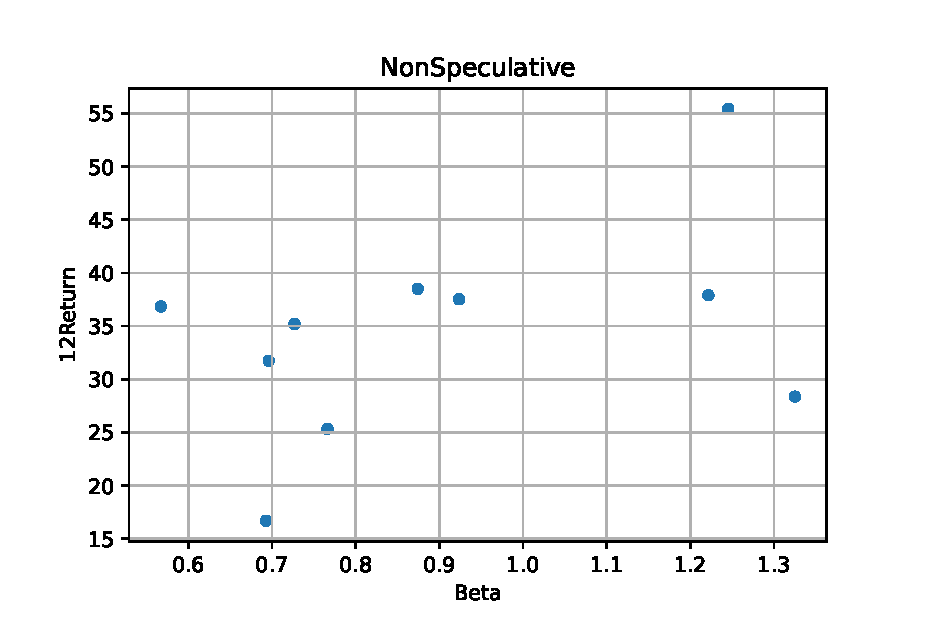
\includegraphics[width=0.7\linewidth]{NonSpeculativeBetaReturn10.eps}
\label{fig:NonSpeculativeBetaReturn10}
\end{figure}




  \FloatBarrier
\section{یافته‌های پژوهش}

با توجه به ادبیات انتظار داریم تا متغیر‌های کنترل گروه، ملاک نقدشوندگی و اندازه تاثیر مثبتی و  انحراف معیار بازده  یکسال گذشته سهام و میزان حق جریان مالی اثر منفی‌ای بر روی هم‌زمانی بازده شرکت داشته باشند. در رابطه اثر نسبت اهرمی نیز در ادبیات هر دو جهت را پیش‌بینی کرده‌است.
 مدل 
\ref{e2}
به وسیله رگرسیون ساده ادغام شده 
\lr{(Pooled OLS)}
با اثر ثابت صنعت و سال برآورد شده‌است. انحراف معیار ضرایب نیز در سطح شرکت‌ها دسته بندی شده است. با توجه به جدول 
\ref{tab:ControlSummary}
ستون آخر آن دسته از مشاهدات که صنعت آن‌ها دارای یک شرکت بوده‌است را از نمونه  برآورد حذف کرده‌ایم و برای حذف اثر تعداد شرکت عضو صنعت نیز متغیر کنترل 
\lr{NOIND}
 را به مدل اضافه کرده‌ایم.
 نتایج برآورد در جدول 
\ref{tab:synchronicityt4}
بیان شده‌است.

ستون شماره 1 نتایج برآورد مدل را به ازای متغیر‌های کنترل نشان می‌دهد. نتایج برآورد نشان می‌دهد که نوسانات گذشته سهم، نسبت اهرم تاثیر چندانی بر روی هم‌زمانی بازده ندارد و برخلاف ادبیات نقدشوندگی و اندازه شرکت در هم‌زمانی بازده شرکت تاثیری به صورت معنا دار منفی دارند. به عبارت دیگر هر آنجه نقدشوندگی سهام یک شرکت کمتر باشد (ملاک 
\lr{Amihud}
بیشتر داشته باشد) اطلاعات مختص شرکت بیشتر در قیمت سهام شرکت وارد می‌شود و از بازار و صنعت خود تاثیر کمتری می‌پذیرد. 
در ستون شماره 2 هم‌زمانی بازده شرکت‌های حاضر در گروه‌های کسب و کار را بر روی متغیر‌های مختص گروه بررسی کرده‌ایم و بر خلاف ادبیات اختلاف حق رای از میزان حق  جریان مالی، تاثیر بیشتری بر روی انعکاس اطلاعات شرکت در قیمت دارد و هم‌زمانی بازده را کاهش می‌دهد که با در نظر گرفتن متغیر‌های کنترل نیز همچنان این اثر وجود دارد.

در سه ستون بعدی نیز به ازای متغیر های گروه دیگر که در بخش قبل تعریف شده‌است بررسی را انجام داده‌ایم و نتایج در جهت برآورد‌های ستون 3 می‌باشد ولی دیگر ضرایب برآورد معنا دار نمی‌باشند. در ستون 7 برآورد را بر روی موقعیت شرکت نسبت به مالک نهایی گروه کسب و کار انجام داده‌ایم و نتایج با نتایج ستون 3 سازگار است. در ستون آخر نیز برآورد را با توجه به مرکزیت شرکت در گروه کسب و کار انجام داده‌ایم. مقایسه نتایج نشان می‌دهد هرآنچه مرکزیت شرکت در گروه کسب و کار بیشتر باشد به این معنا که مالک نهایی بتواند از شرکت برای کنترل بر دیگر اعضای گروه استفاده کند، اطلاعات مختص شرکت در قیمت شرکت منعکس نمی‌شود.

یکی از نگرانی‌های احتمالی با توجه به 
رگرسیون ساده ادغام شده 
\lr{(Pooled OLS)}
وجود وابستگی میان بخشی است که در برآورد‌های انجام شده تا کنون این خطا اصلاح نشده‌است. به همین علت در ادامه تمامی مدل‌های جدول
\ref{tab:synchronicityt4}
را به وسیله شیوه دو مرحله‌ای 
فاما و مکبث 
	\lr{(Fama and MacBeth)}
	تکرار کرده‌ایم و انحراف معیار‌های این برآورد را با در نظر گرفتن واریانس ناهمسانی و همبستگی با خود 
	\lr{(Auto-correlation)}
	به روش نیوی و وست
	\lr{(Newey and West)}
	برای 4 سال اصلاح شده‌است. نتایج برآورد در جدول 
	\ref{tab:synchronicityt5}
	گزارش شده است که به صورت کلی با جدول 
	\ref{tab:synchronicityt4} 
	سازگار است. متغیر‌های کنترل اختلاف حق‌ رای از حق مالی  در این حالت در حضور متغیر‌های کنترل دیگر اهمیت خود را از دست می‌دهند و همچنان متغیر مرکزیت شرکت در گروه در جهت افزایش هم‌زمانی و کاهش نقش اطلاعات مختص شرکت در قیمت شرکت  تاثیر می‌گذارد. در این روش  برآورد برخلاف روش قبل نوسانات گذشته شرکت نیز در هم‌زمانی بازده تاثیر مثبت ایفا می‌کند.

نتایج جدول 
\ref{tab:synchronicityt4} 
و
\ref{tab:synchronicityt5} 
نشان می‌دهد برخلاف مقاله بوباکر و همکاران  (2014)
%\lr{(\cite{boubaker2014large})}
توزیع حق کنترل و حق جریان در شرکت رفتار بازده شرکت را توضیح نمی‌دهد و به عبارت دیگر اختلاف حق رای و حق جریان مالی مانعی در برابر تاثیر اطلاعات شرکت در قیمت شرکت نیست اما از طرفی چنانچه شرکت دارای مرکزیت بالاتری در گروه کسب و کار باشد در این صورت این مانع وجود دارد و سبب می‌شود تا هم‌زمانی بازده شرکت با بازار و صنعت افزایش پیدا کنید که به نظر می‌آید نتیجه‌ای جدید در این ادبیات باشد. 



%				\begin{table}[htbp]
%	\centering
%	\caption{نتایج برآورد مدل \ref{e2}
%	به ازای متغیر‌های مختلف کنترل به روش 
%\lr{(Pooled OLS)}
%}
%	\resizebox{0.7\textheight}{!}{
%\lr{		\input{synchronicityt4.tex}
%		\label{tab:synchronicityt4}	
%	}
%}
%\end{table}



 
%	\begin{table}[htbp]
%	\centering
%\caption{نتایج برآورد مدل \ref{e2}
%	به ازای متغیر‌های مختلف کنترل به روش 
%	\lr{(Fama and MacBeth)}
%}
%	\lr{	\resizebox{0.7\textheight}{!}{
%			\input{synchronicityt5.tex}
%			\label{tab:synchronicityt5}	
%		}}
%	\end{table}


\FloatBarrier

\section{نتیجه‌گیری و پیشنهاد‌ها}

\begin{LTR}		
	\bibliographystyle{apalike}
	\bibliography{Ref}
\end{LTR}
\end{document}